Als we binnen Event Viewer naar de \textquote{Windows Logs} gaan en daar klikken op \textquote{System} dan zien we er alle meldingen van het systeem die vastgelegd zijn. Dubbelklikken we op een Event dan krijgen we meer uitgebreidde informatie.

\begin{minipage}[t]{\linewidth}
\raggedright
\adjustbox{valign=t}{%
	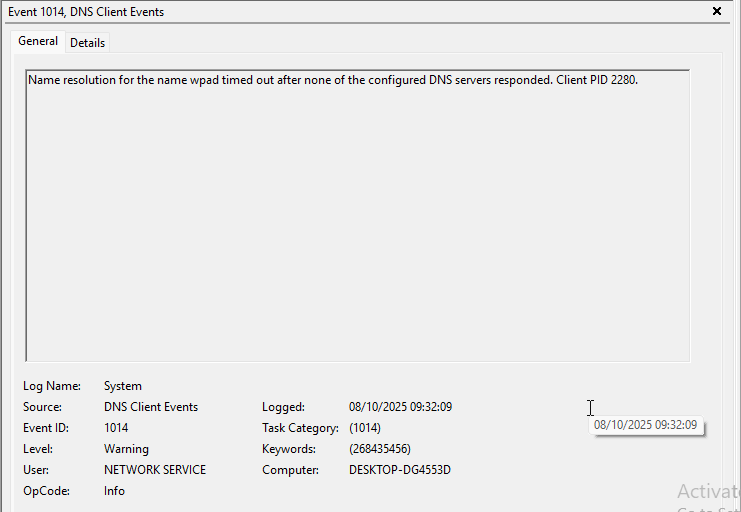
\includegraphics[width=0.99\linewidth]{ev-event.png}%
}
\end{minipage}

Bij dit event zien we een aantal verschillende velden onder de mededeling. Een aantal van deze velden zijn voor ons van belang:
\begin{description}
\item[Logged] geeft de datum en tijd waarop het event is binnengekomen
\item[Source] vertelt ons iets over de herkomst van het event
\item[Event ID] is een nummer dat ons kan helpen bij het vinden van nadere informatie. Via een Internet Zoekmachine kunnen we zoeken op de Event ID en zo meer informatie verzamelen over het gebeurde. Het beste is om te zoeken naar \textquote{Windows Event ID <nummer>}
\item[Level] geeft aan hoe belangrijk een event is. Er zijn verschillende levels:
	\begin{description}
	\item[Critical] Dit zijn meldingen waarop direct gereageerd zou moeten worden.
	\item[Error] Problemen die optreden, maar die kritiek zijn.
	\item[Warning] Waarschuwingen die een indicatie kunnen zijn dat er een probleem zit aan te komen. Zouden nader onderzocht moeten worden om problemen voor te zijn.
	\item[Information] Informatie die handig is om te weten, maar die geen probleem aangeven.
	\item[Verbose] Informatie die voortgang of succes meldingen zijn. Kunnen over het algemeen genegeerd worden.
	\end{description}
\end{description}

